%!TEX root = ../paper.tex
\section{Web Application}
\label{sec:web}

A web-based interface serves as an easily accessible interface to our classification system.
Users are given the opportunity to upload a video file as input for the prediction.
Alternatively, we provide example videos from the UCF-101 dataset for quick access.
The uploaded video material undergoes the same preprocessing as outlined in section \ref{sec:data}.
The extracted frames and optical flows serve as the input for the spatial and temporal network, respectively.
The joint prediction results are returned by means of a REST interface and are presented two-fold as shown in figure \ref{fig:web_app}:
\textit{(1)} Next to a preview of the video is the overall classification summary given by the top five label probabilities.
(\textit{2}) To reflect a video’s temporal dimension the demo presents a per-frame based evaluation highlighting the top five probabilities for each frame.
For easy verification a click on the graphical nodes synchronizes the preview video with the selected frame.

\begin{figure}[!htb]
	\centering
	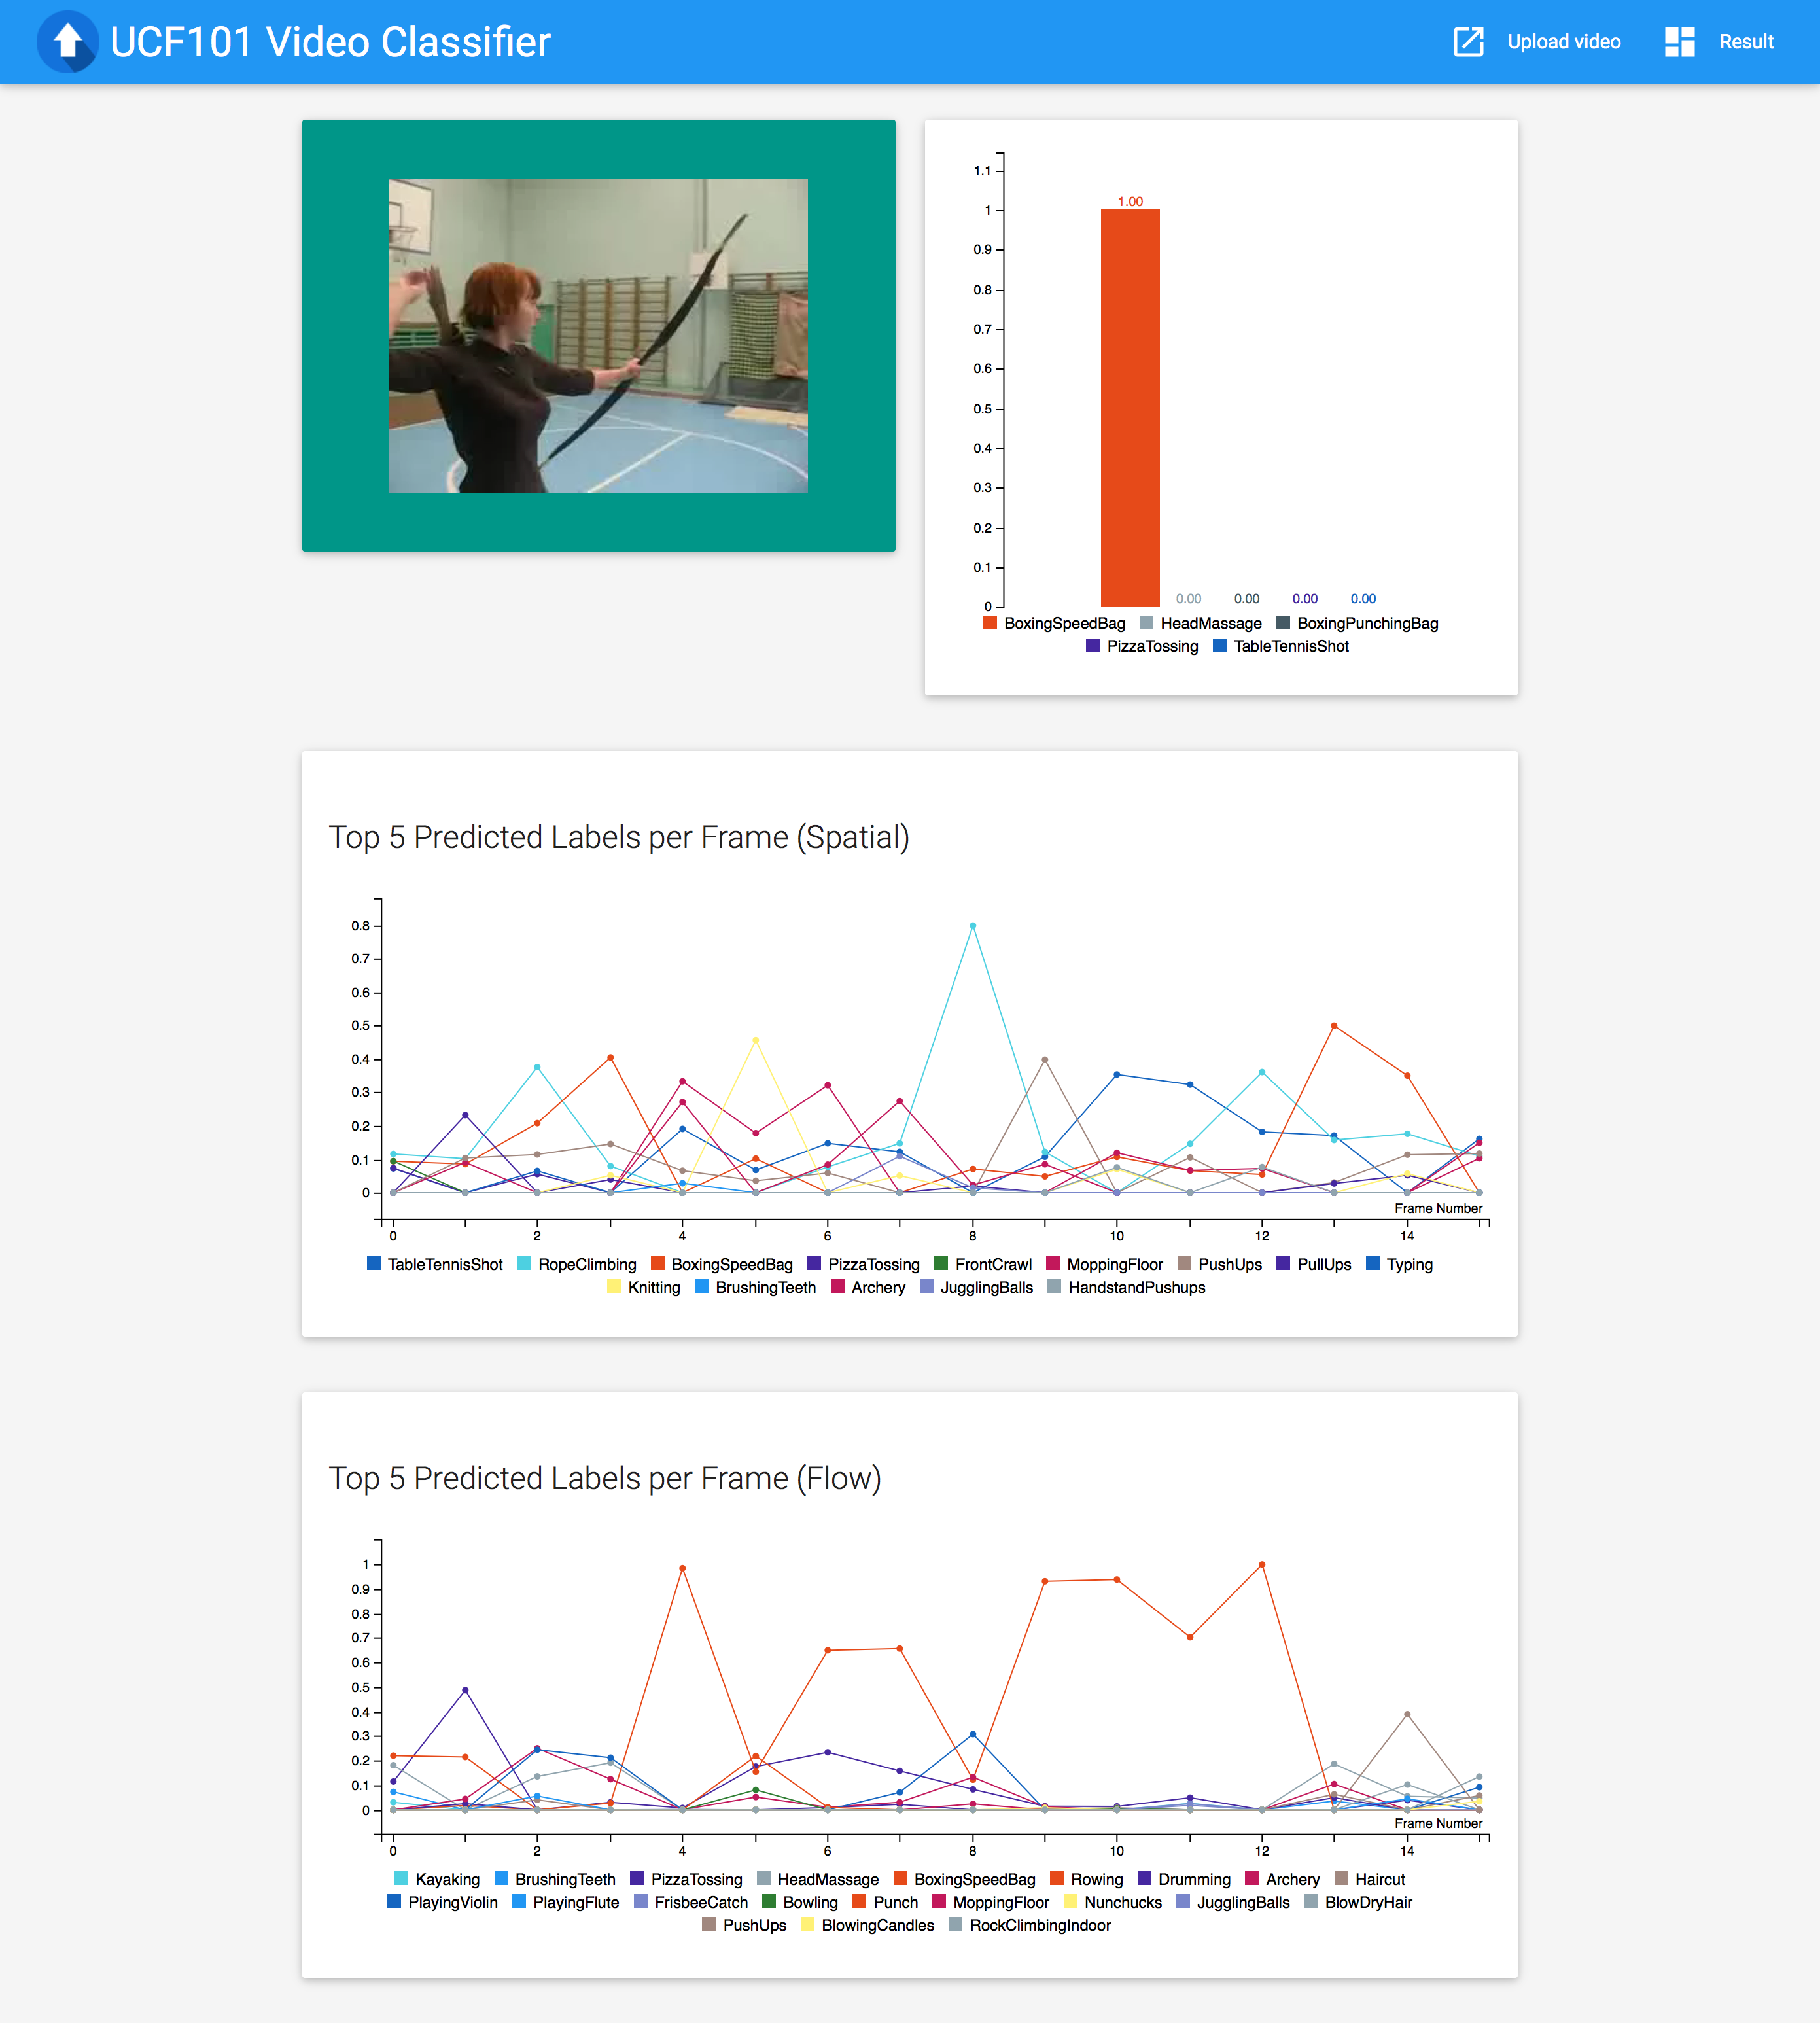
\includegraphics[width=0.9\textwidth]{images/screenshot.png}
	\caption{Visualization of the network's results: (Top) The video with the overall classification summary given by the top five label probabilities is given. (Middle) The per frame prediction of the \emph{spatial} neural network. (Bottom) The per frame prediction of the \emph{flow} neural network is shown.}
	\label{fig:web_app}
\end{figure}

\subsection{Architecture}
The system contains of two almost independent parts:
(\textit{1}) A modern single-page web app.
The frontend utilizes the modular \textit{React}\footnote{\url{https://facebook.github.io/react}} UI-framework and follows the \textit{Flux} \footnote{\url{https://facebook.github.io/flux}} unidirectional data flow pattern.
Frontend routing, templating and interaction handling provides a rich and seamless experience.
In order to utilize the latest Javascript ES6 language-level features and retain backward compatibility with older browsers the frontend part has to be transpiled into a single file.
The scriptable module bundler \textit{Webpack} \footnote{\url{https://webpack.github.io}} takes care of that.

\textit{(2)} The server part is implemented in the Flask framework \footnote{\url{http://flask.pocoo.org}} for Python.
Besides providing an easy to modify web framework our choice for Python makes it easy to include Caffe through the PyCaffe bindings.
User videos are locally preproccessed using the same FFmpeg and OpenCV pipeline as outlined previously in section \ref{sec:data}.
After initially serving the web app to a client, all communication is then through a REST interface.

\subsection{Setup}
Make sure to install NodeJS, Python 2.7, OpenCV, PyCaffe and FFmpeg.
Listing \ref{lst:web-app} shows the required commands to install all further dependencies and run the server.

\begin{lstlisting}[language=sh, caption=Web Application Setup, label=lst:web-app]
cd web-server

# frontend dependencies
npm install -g webpack
npm install
npm run build

#server dependencies
pip install -r requirements.txt

#run the server
python server.py
\end{lstlisting}